


\documentclass{article}

\usepackage{graphicx} 
\begin{document}

\section{Autonomes Erkunden}
\label{subsec:autonomeserkunden}
Das autonome Erkunden kann man in drei grundlegende Teilgebiete gliedern. An erster Stelle steht das ROS-Paket Gmapping\footnote{http://wiki.ros.org/gmapping}, welches für die Lokalisierung des Autos im Raum, sowie dem schrittweisen Kartographieren der Umgebung zuständig ist. Aus den Daten des Gmapping kann dann das Automap Paket berechnen, wohin das Auto fahren soll, um die Umgebung komplett und durch möglichst einfache Lenkmanöver erkunden zu können. Und letztendlich benötigt man einen funktionierenden Navigation Stack, der diese Ziele dann entgegennimmt und die Steuerbefehle für das Auto erzeugt. 

\subsection{Gmapping}
\label{subsec:gmapping}
Der große Unterschied hierbei zu den vorangehenden Aufgaben liegt darin, dass beim Erkunden keine statische Karte vorgegeben ist, sondern man ohne Anhaltspunkte startet und sich die Umgebung Stück für Stück zusammensetzt, d.h. sich mit jeder Bewegung des Fahrzeuges ändert. Zum Bewältigen dieser komplexen Aufgabe kommt das Gmapping Paket zum Einsatz. Neben dem Erstellen der Karte besteht die andere Aufgabe des Gmapping noch darin, die aktuelle Position des Autos auf der Karte zu bestimmen. Da beide Aufgaben parallel ablaufen ist der mapping Algoritmus auch häufig unter dem erweiterteten Begriff SLAM Gmapping anzutreffen, wobei SLAM für Simultaneous Localization and Mapping steht. Als Input benötigt das Paket den Laserscan der Kinect und die Odometriedaten des Autos. Der Laserscan wird in unserem Fall noch durch einen Filter verbessert, was in (Kapitel Lokalisierung--Tiefenbild der Kinect) erwähnt wird. Mit jedem Eintreffen von neuen Daten kann nun der Algorithmus mit den bisherigen Werten vergleichen und die Karte aktualisieren bzw die aktuelle Position darin schätzen. Dies funktioniert auch mit ziemlich guter Genauigkeit sofern sich das Auto in Gebieten mit vielen Anhaltspunkten, wie z.B. viele Kanten zur Orientierung, befindet. Sobald man allerdings auf offen gelegene Gebiete zufährt, zeigt sich der Algorithmus allerdings häufig fehleranfällig und liefert nicht immer gute Ergebnisse. Das resultiert dann in verrutschten Kanten auf der Karte (Skizze.....) und Positionssprüngen. Um dies entgegenzuwirken, kann man am Algorithmus unzählige Paramtereinstellungen vornehmen, so dass schätzungsweiße ungenaue Laserscans verworfen werden, welche immer dann eintreffen, wenn man gerade eine große offene Fläche entdeckt hat. Weiterhin kann man genauere Ergebnisse erzielen, wenn man die Update Raten (=mehr Inputdaten) für das Verarbeiten der eingehenden Laserscans erhöht. In dem Fall steigt die Genauigkeit auf Kosten der Performance, welches speziell in Kombination mit dem Automap Algorithmus eine Rolle spielt und in (subsection Probleme) weiter erläutert wird. 
\begin{figure}[h]
  \centering
     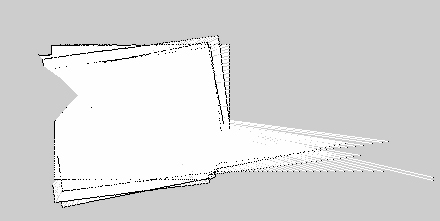
\includegraphics[width=1.0\textwidth]{Includes/gmap.jpg}
  \caption{verrutschte Kanten beim Gmapping}
  \label{fig:Mapping}
\end{figure}

\subsection{Automap}
\label{subsec:automap}
Das Automap Paket wurde von Sebastian Ehmes, vorjähriger Teilnehmer des Projektseminar Echtzeitsysteme und Betreuer für das diesjährige Projektseminar, im Rahmen seiner Bachelorarbeit entwickelt und ist verantwortlich für die eigentliche Erkundungsstategie. Wenn man einen Schnappschuss (Ergebnis Gmapping, Skizze....) betrachtet, hat man auf der einen Seite das bereits bekannte Terrain und auf der anderen Seite Grenzen, die an unbekannten Gebieten anliegen. Im ersten Schritt findet nun der Automap Algorithmus alle solche Grenzen auf der bisher aufgezeichneten Karte, um dann im zweiten Schritt zu berechnen, welche dieser Grenzen am kostengünstigen angefahren werden kann. In unserem Fall bedeutet dies, dass Ziele in Fahrtrichtung bevorzugt werden, da unser Auto aufgrund der Ackermann Lenkung in seiner Mobilität eingeschränkt ist und große Wendemanöver sehr aufwendig sind. Da sich die Karte mit jeder Bewegung des Fahrzeugs ändern kann und sich wiederum auch die Grenzen verschieben, können aktuelle Anfahrtsziele vorzeitig abgebrochen werden und der Automap Algorithmus berechnet erneut die optimale Route. Das Automap Paket konnte sehr gut in unser Projekt integriert werden, da sich viele unserer Ansätze mit denen aus Sebastians Bachelorarbeit gedeckt haben, so z.B. die Benutzung von Gmapping und der Aufbau des Navigation Stacks, währenddessen sich die Integration anderer ROS Pakete, welche einen Erkundungsalgorithmus implementieren, als schwierig erwießen hat, da diese teils andere Voraussetzungen (holonome Roboter statt Ackermann Modell) erwarteten.

\subsection{Navigation Stack}
\label{subsec:navigationstack}
Der Navigation Stack hat die Aufgabe die eigentlichen Motor bzw Lenkbefehle an das Auto zu senden. Dafür benötigt man zuerst einmal die Information wohin das Fahrzeug fahren soll, was über das Automapping (subsection Automap) geschieht und außerdem eine Pfaderstellung vom aktuellem Standpunkt des Fahrzeugs zum Zielort, welches mit Hilfe eines globalen bzw lokalen Planners erfolgt. Die Funktionsweiße der Planner gleicht der aus dem Kapitel (Verweise...), weshalb hier nicht weiter darauf eingegangen wird. Während beim Rundkurs mit Hinternissen die Zielposition stehts fest vorgegeben war, muss diese beim autonomen Erkunden ständig angepasst werden und darin liegt auch der größte Unterschied der beiden Disziplinen. 

\subsection{Probleme}
\label{subsec:probleme}
Wie schon bereits in (subsection Gmapping) angedeutet, spielt die Balance zwischen Qualität des Endproduktes (gezeichnete Karte) und Performance eine wesentliche Rolle. So haben wir häufig die Fälle gehabt, dass unser Auto während des Erkundens entweder seine Position verloren hat (Fokus: Performance>Qualität), oder die Algorithmen mit der Menge an Daten nicht klargekommen ist und das Auto auf der Stelle verharrte(Fokus: Qualität>Performance). Das Finden der optimalen Parameterwerte für die jeweiligen Pakete ist eine Kunst für sich und hatte den Trend Unmengen an Zeit zu verschlingen. Während das Erkunden von kleinen abgeschlossen Räumen noch funktioniert hat, konnten wir das selbe Ergebnis nicht für weitläufigere Gebiete reproduzieren, letztendlich fehlte dafür einfach die Zeit.
\end{document}


